\documentclass[tikz,margin=5pt]{standalone}
\usepackage{tikz}
\usepackage{pgfplots}
\pgfplotsset{compat=1.16}

%\usepackage{newtxtext}
%\usepackage{newtxmath}
\usepackage{mathpazo}

\usepackage{graphicx}

\begin{document}

\begin{tikzpicture}
  \node at (0, 0) {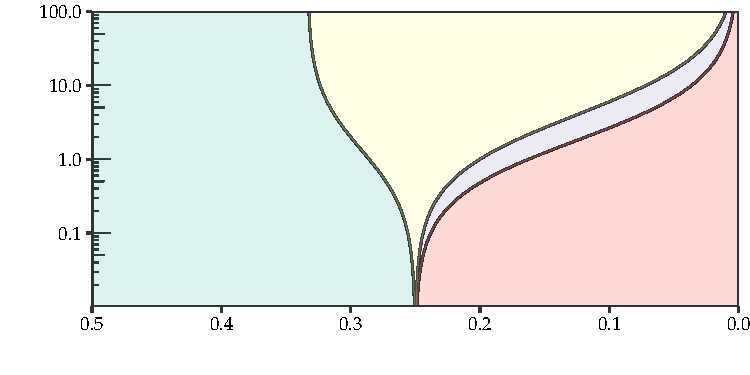
\includegraphics[scale=0.8]{../Rsession/phases.pdf}};
  \node at (-3, -5.5) {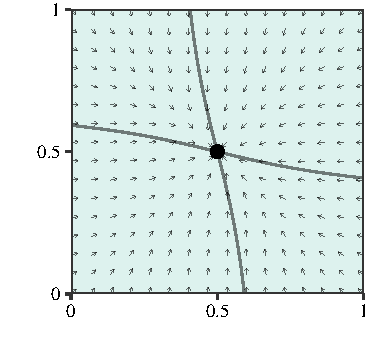
\includegraphics[scale=0.8]{../Rsession/phaseI.pdf}};
  \node at (-3, 5.5) {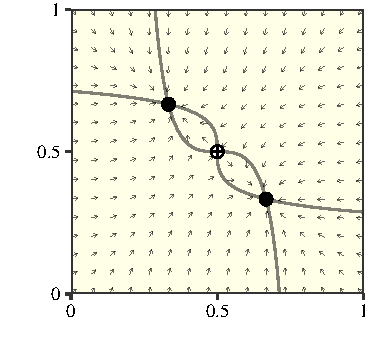
\includegraphics[scale=0.8]{../Rsession/phaseII.pdf}};
  \node at (3.3, 5.5) {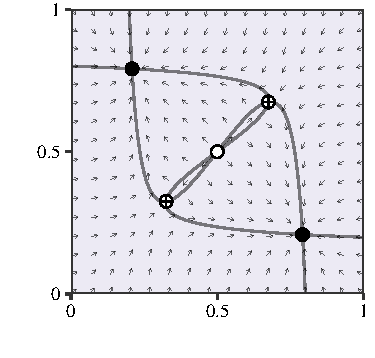
\includegraphics[scale=0.8]{../Rsession/phaseIII.pdf}};
  \node at (3.3, -5.5) {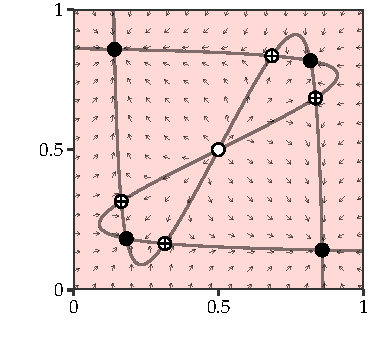
\includegraphics[scale=0.8]{../Rsession/phaseIV.pdf}};

  \node[below] at (-2.55, 3.5) {$x_1$};
  \node[below] at (-2.55 + 6.3, 3.5) {$x_1$};
  \node[below] at (-2.55, -7.5) {$x_1$};
  \node[below] at (-2.55 + 6.3, -7.5) {$x_1$};

  \node[left] at (-5.1, 5.85) {$x_2$};
  \node[left] at (-5.1 + 6.3, 5.85) {$x_2$};
  \node[left] at (-5.1, -5.12) {$x_2$};
  \node[left] at (-5.1 + 6.3, -5.12) {$x_2$};

  \node[below] at (0.5, -2.1) {$\mu$};
  \node[left] at (-4.60, 0.35) {$\sigma$};

  \draw (-1.2, 0.4) -- (-1.6, -3.2);
  \draw (0.5, 0.4) -- (-1.6, 3.99);
  \draw (1.8, 0.4) -- (2.8, 3.99);
  \draw (2.7, 0.4) -- (2.8, -3.2);

  \node at (-2.0, 0.3) {\large I};
  \node at (1.1, 1.3) {\large II};
  \node at (2.7, 0.8) {\large III};
  \node at (3.8, -0.4) {\large IV};

  \node[above] at (-1.7, 2.5) {$\mu_3$};
  \node[above] at (4.0, 2.5) {$\mu_2$};
  \node[above] at (5.6, 2.5) {$\mu_1$};
  \draw (-1.5, 2.6) -- (-0.91, 2.38);
  \draw (4.2, 2.6) -- (4.75, 2.38);
  \draw (5.4, 2.6) -- (4.84, 2.38);

\end{tikzpicture}
\end{document}

